\chapter{Membangun Model Prediksi}

Untuk pratikum saati ini menggunakan buku \textit{Python Artificial Intelligence Projects for Beginners}\cite{eckroth2018python}. Dengan praktek menggunakan python 3 dan editor anaconda dan library python scikit-learn.
Dataset ada di https://github.com/PacktPublishing/Python-Artificial-Intelligence-Projects-for-Beginners .
Tujuan pembelajaran pada pertemuan pertama antara lain:
\begin{enumerate}
	\item
	      Mengerti implementasi klasifikasi
	\item
	      Memahami data set, training dan testing data
	\item
	      Memahami Decission tree.
	\item
	      Memahami information gain dan entropi.
\end{enumerate}
Tugas dengan cara dikumpulkan dengan pull request ke github dengan menggunakan latex pada repo yang dibuat oleh asisten riset. Kode program menggunakan input listing ditaruh di folder src ekstensi .py dan dipanggil ke latex dengan input listings. Tulisan dan kode tidak boleh plagiat, menggunakan bahasa indonesia yang sesuai dengan gaya bahasa buku teks.

\section{Teori}
Praktek teori penunjang yang dikerjakan(nilai 5 per nomor, untuk hari pertama) :
\begin{enumerate}
	\item
	      Jelaskan apa itu binary classification dilengkapi ilustrasi gambar sendiri \\
	      \textbf{Binary Classification} merupakan Klasifikasi biner yang berupa kelas positifi atau negatif yang di tetapkan untuk tujuan yang praktis dari pada akurasi keseluruhan serta relatif dari berbagai jenis kesalahan yang menarik.\\

	      Contoh: mendeteksi penyakit ketika tidak ada(false positive), tidak mendeteksi penyakit ketika hadir(false negative)
	\item
	      Jelaskan apa itu supervised learning dan unsupervised learning dan clustering dengan ilustrasi gambar sendiri.
	\item
	      Jelaskan apa itu evaluasi dan akurasi dari buku dan disertai ilustrasi contoh dengan gambar sendiri.\\
	      \textbf{Evaluasi dan Akurasi} Evaluasi untuk mengukur akurasi model bekerja, dan akurasi persentase klasifikasi dengan benar.
	\item
	      Jelaskan bagaimana cara membuat dan membaca confusion matrix, buat confusion matrix buatan sendiri.
	\item
	      Jelaskan bagaimana K-fold cross validation bekerja dengan gambar ilustrasi contoh buatan sendiri.
	\item
	      Jelaskan apa itu decision tree dengan gambar ilustrasi contoh buatan sendiri.\\
	      \textbf{Decision Tree} Digunakan untuk klasifikasi dan regresi dengan menggunakan metode pembelajaran non-parametrik yang dapat menghasilkan nilai puput berupa model yang memprediksi nilai variable target dengan aturan keputusan dari fitur data.
	\item
	      Jelaskan apa itu information gain dan entropi dengan gambar ilustrasi buatan sendiri.\\
	      \textbf{Information Gain} merupakan penurunan entropi setelah dataset di bagi  pada atribut serta membangun decision tree untuk menemukan atribut yang mengembalikan informasi krusial(cabang paling homogen).\\
	      \textbf{Entropi} merupakan tingkat keacakan dalam informasi, semakin tinggi entropi semakin sulit menyumpulkan dari informasi yang acak. begitupun sebaliknya.
\end{enumerate}

\section{scikit-learn}
Dataset ambil di https://github.com/PacktPublishing/Python-Artificial-Intelligence-Projects-for-Beginners folder Chapter01.
Tugas anda adalah, dataset ganti menggunakan \textbf{student-mat.csv} dan mengganti semua nama variabel dari kode di bawah ini dengan nama-nama makanan (NPM mod 3=0), kota (NPM mod 3=1), buah (NPM mod 3=2), . Jalankan satu per satu kode tersebut di spyder dengan menggunakan textit{Run current cell}. Kemudian Jelaskan dengan menggunakan bahasa yang mudah dimengerti dan bebas plagiat dan wajib skrinsut dari komputer sendiri masing masing nomor di bawah ini(nilai 5 masing masing pada hari kedua).

\paragraph{\textbf Youtube :}

\begin{enumerate}

	\item
	      \begin{verbatim}
	# load dataset (student mat pakenya)
	import pandas as pd
	d = pd.read_csv('student-mat.csv', sep=';')
	len(d)
\end{verbatim}
	      \begin{figure}[ht]
		      \centerline{\includegraphics[scale=0.7]{figures/Chapter2a.png}}
		      \caption{Load dataset}
		      \label{Load dataset}
	      \end{figure}

	\item
	      \begin{verbatim}
	# generate binary label (pass/fail) based on G1+G2+G3 
	# (test grades, each 0-20 pts); threshold for passing is sum>=30
	d['pass'] = d.apply(lambda row: 1 if (row['G1']+row['G2']+row['G3']) 
											>= 35 else 0, axis=1)
	d = d.drop(['G1', 'G2', 'G3'], axis=1)
	d.head()
\end{verbatim}
	      \begin{figure}[ht]
		      \centerline{\includegraphics[scale=0.7]{figures/Chapter2b.png}}
		      \caption{Generate binary label}
		      \label{Generate binary label}
	      \end{figure}

	\item
	      \begin{verbatim}
	# use one-hot encoding on categorical columns
	d = pd.get_dummies(d, columns=['sex', 'school', 'address', 
									'famsize', 
									'Pstatus', 'Mjob', 'Fjob', 
	                               'reason', 'guardian', 'schoolsup', 
								   'famsup', 'paid', 'activities',
	                               'nursery', 'higher', 'internet', 
									'romantic'])
	d.head()
\end{verbatim}
	      \begin{figure}[ht]
		      \centerline{\includegraphics[scale=0.7]{figures/Chapter2c.png}}
		      \caption{Generate binary label}
		      \label{Generate binary label}
	      \end{figure}

	      \newpage
	\item
	      \begin{verbatim}
	# shuffle rows
	d = d.sample(frac=1)
	# split training and testing data
	d_train = d[:500]
	d_test = d[500:]

	d_train_att = d_train.drop(['pass'], axis=1)
	d_train_pass = d_train['pass']

	d_test_att = d_test.drop(['pass'], axis=1)
	d_test_pass = d_test['pass']

	d_att = d.drop(['pass'], axis=1)
	d_pass = d['pass']

	
\end{verbatim}
	      \begin{figure}[ht]
		      \centerline{\includegraphics[scale=0.7]{figures/Chapter2d.png}}
		      \caption{Shuffle row}
		      \label{Shuffle row}
	      \end{figure}

	      \begin{verbatim}
	# number of passing students in whole dataset:
	import numpy as np
	print("Passing: %d out of %d (%.2f%%)" % (np.sum(d_pass), len(d_pass), 
	       100*float(np.sum(d_pass)) / len(d_pass)))
\end{verbatim}
	      \begin{figure}[ht]
		      \centerline{\includegraphics[scale=0.7]{figures/Chapter2e.png}}
		      \caption{Number of passing}
		      \label{Number of passing}
	      \end{figure}

	      \newpage

	\item
	      \begin{verbatim}
	# fit a decision tree
	from sklearn import tree
	t = tree.DecisionTreeClassifier(criterion="entropy", max_depth=5)
	t = t.fit(d_train_att, d_train_pass)
\end{verbatim}
	      \begin{figure}[ht]
		      \centerline{\includegraphics[scale=0.7]{figures/Chapter2f.png}}
		      \caption{Fit a decision tree}
		      \label{Fit a decision tree}
	      \end{figure}

	\item
	      \begin{verbatim}
	# visualize tree
	import graphviz
	dot_data = tree.export_graphviz(t, out_file=None, label="all", 
									impurity=False, proportion=True,
	                                feature_names=list(d_train_att), 
									class_names=["fail", "pass"], 
	                                filled=True, rounded=True)
	graph = graphviz.Source(dot_data)
	graph
\end{verbatim}
	      \begin{figure}[ht]
		      \centerline{\includegraphics[scale=0.7]{figures/Chapter2g.png}}
		      \caption{Visualize tree}
		      \label{Visualize tree}
	      \end{figure}

	\item
	      \begin{verbatim}
	# save tree
	tree.export_graphviz(t, out_file="student-performance.dot", 
						 label="all", impurity=False, 
						 proportion=True,
	                     feature_names=list(d_train_att), 
	                     class_names=["fail", "pass"], 
	                     filled=True, rounded=True)
\end{verbatim}
	      \begin{figure}[ht]
		      \centerline{\includegraphics[scale=0.7]{figures/Chapter2h.png}}
		      \centerline{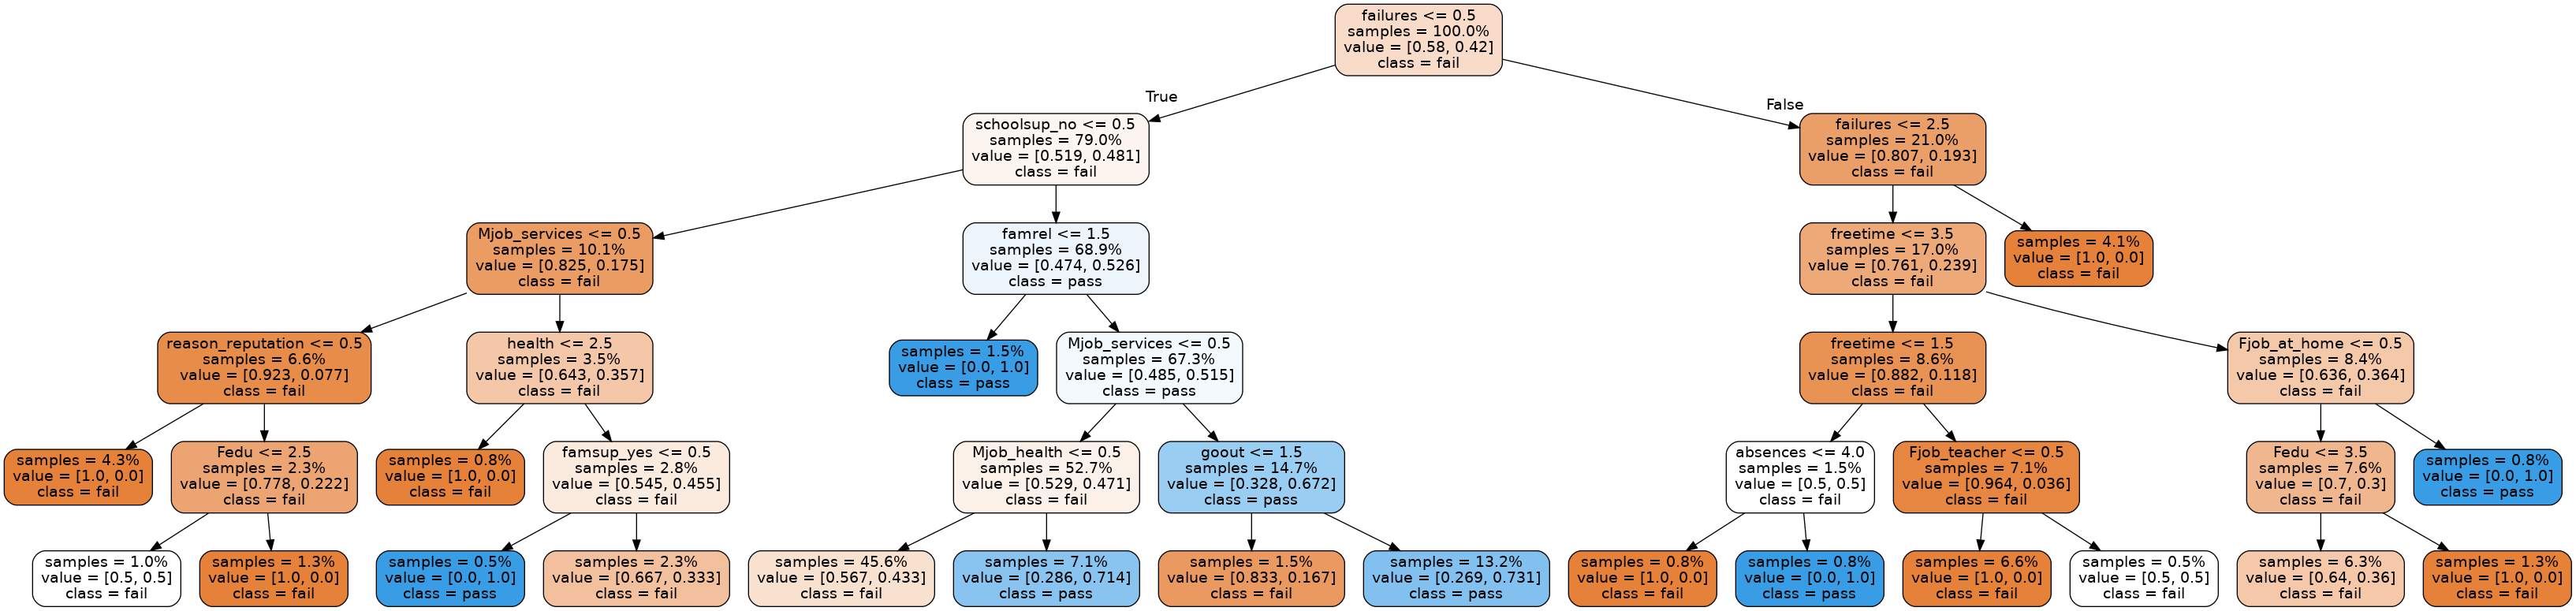
\includegraphics[scale=0.1]{figures/student-performance.png}}
		      \caption{Save tree dot to png}
		      \label{Save tree dot to png}
	      \end{figure}

	\item
	      \begin{verbatim}
	t.score(d_test_att, d_test_pass)
\end{verbatim}
	      \begin{figure}[ht]
		      \centerline{\includegraphics[scale=0.7]{figures/Chapter2i.png}}
		      \caption{scores}
		      \label{scores}
	      \end{figure}

	\item
	      \begin{verbatim}
	from sklearn.model_selection import cross_val_score
	scores = cross_val_score(t, d_att, d_pass, cv=5)
	
\end{verbatim}
	      \begin{figure}[ht]
		      \centerline{\includegraphics[scale=0.7]{figures/Chapter2j.png}}
		      \caption{scores II}
		      \label{scores II}
	      \end{figure}

	      \begin{verbatim}
	# show average score and +/- two standard deviations away 
	#(covering 95% of scores)
	print("Accuracy: %0.2f (+/- %0.2f)" % (scores.mean(), scores.std() * 2))
\end{verbatim}
	      \begin{figure}[ht]
		      \centerline{\includegraphics[scale=0.7]{figures/Chapter2k.png}}
		      \caption{Show average score}
		      \label{Show average score}
	      \end{figure}

	\item
	      \begin{verbatim}
	for max_depth in range(1, 20):
	    t = tree.DecisionTreeClassifier(criterion="entropy", 
			max_depth=max_depth)
	    scores = cross_val_score(t, d_att, d_pass, cv=5)
	    print("Max depth: %d, Accuracy: %0.2f (+/- %0.2f)" % 
				(max_depth, scores.mean(), scores.std() * 2)
			 )
\end{verbatim}
	      \begin{figure}[ht]
		      \centerline{\includegraphics[scale=0.7]{figures/Chapter2l.png}}
		      \caption{DecisionTreeClassifier}
		      \label{DecisionTreeClassifier}
	      \end{figure}

	\item
	      \begin{verbatim}
	depth_acc = np.empty((19,3), float)
	i = 0
	for max_depth in range(1, 20):
	    t = tree.DecisionTreeClassifier(criterion="entropy", 
			max_depth=max_depth)
	    scores = cross_val_score(t, d_att, d_pass, cv=5)
	    depth_acc[i,0] = max_depth
	    depth_acc[i,1] = scores.mean()
	    depth_acc[i,2] = scores.std() * 2
	    i += 1

	depth_acc
\end{verbatim}

	      \newpage

	      \begin{figure}[ht]
		      \centerline{\includegraphics[scale=0.7]{figures/Chapter2m.png}}
		      \caption{DecisionTreeClassifier depth}
		      \label{DecisionTreeClassifier depth}
	      \end{figure}

	\item
	      \begin{verbatim}
	import matplotlib.pyplot as plt
	fig, ax = plt.subplots()
	ax.errorbar(depth_acc[:,0], depth_acc[:,1], yerr=depth_acc[:,2])
	plt.show()
\end{verbatim}
	      \begin{figure}[ht]
		      \centerline{\includegraphics[scale=0.6]{figures/Chapter2n.png}}
		      \caption{Subplots}
		      \label{Subplots}
	      \end{figure}

\end{enumerate}

\newpage

\section{Penanganan Error}
Dari percobaan yang dilakukan di atas, error yang kita dapatkan di dokumentasikan dan di selesaikan(nilai 5 hari kedua):

\begin{enumerate}
	\item
	      skrinsut error
	\item
	      Tuliskan kode eror dan jenis errornya
	\item
	      Solusi pemecahan masalah error tersebut

\end{enumerate}

